\documentclass[12pt,a4paper]{article}
\usepackage[utf8]{inputenc}
\usepackage[english]{babel}
\usepackage[T1]{fontenc}

\usepackage{lmodern}

\usepackage{url}
\usepackage{hyperref}
\hypersetup{colorlinks=true,urlcolor=blue}

\usepackage{graphicx}

\usepackage[top=3cm, bottom=3cm, left=2.5cm, right=2.5cm]{geometry}

\setlength\parindent{0pt}

\author{Florent Hédin}
\title{FittingWizard : Status of the current implementation}

\begin{document}

\maketitle

\tableofcontents

\section{Overview of the workflow for the current version}

\subsection{Welcome screen}

At initial run, welcome screen for choosing what to do : Figure \ref{fig0} \\

%\medskip

\begin{figure}[h!]
\centering
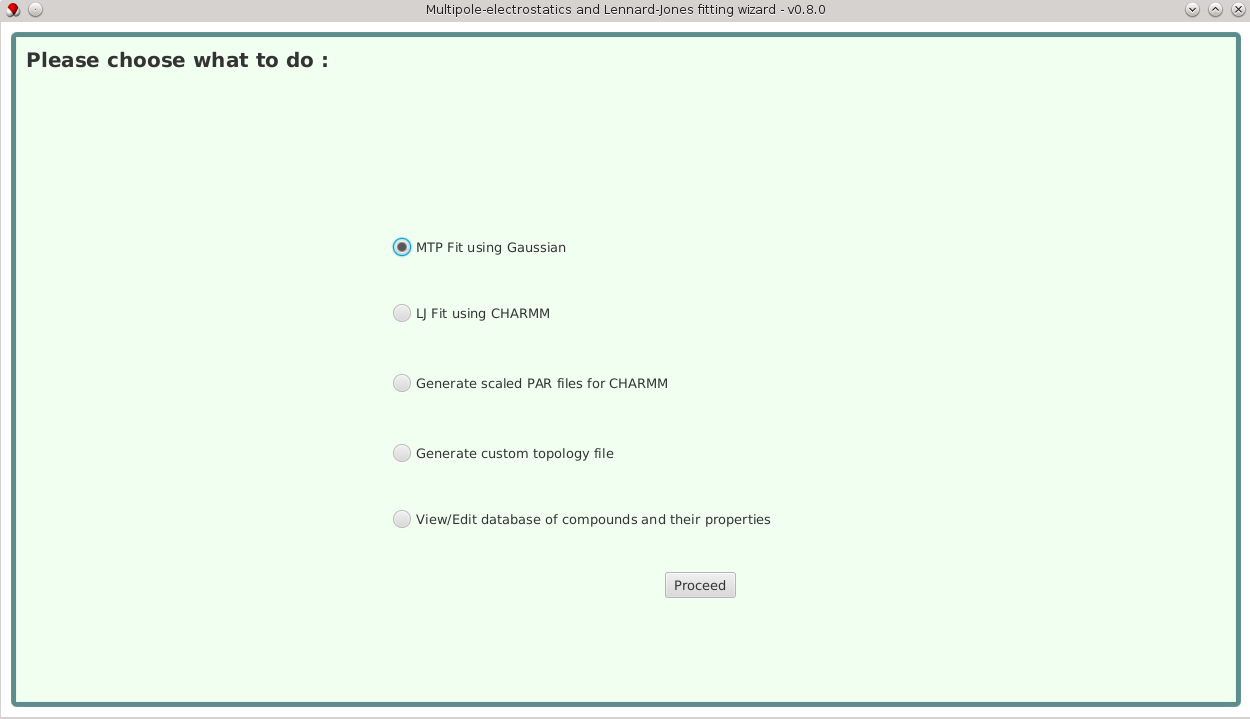
\includegraphics[width=0.9\linewidth]{pics/scr0}
\caption{Welcome screen}
\label{fig0}
\end{figure}

\subsection{MTP parameters from Ab Initio}

\subsubsection{Loading coordinates}

First selection in welcome screen gives access to the Gaussian optimization procedure, where first 
a molecule 
is loaded : Figure \ref{fig1} \\

%\medskip

\begin{figure}[h!]
\centering
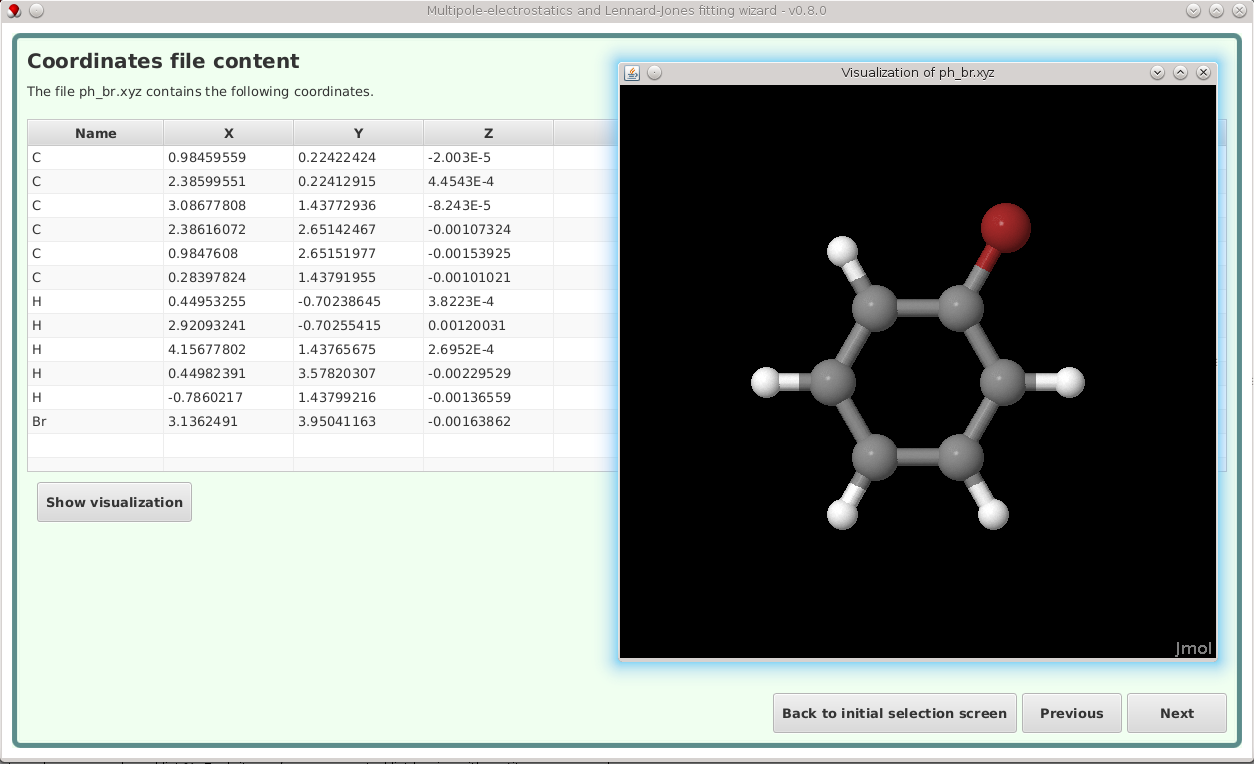
\includegraphics[width=0.9\linewidth]{pics/scr1}
\caption{Loading molecule}
\label{fig1}
\end{figure}

\subsubsection{MTP fit}

Then after success of the Ab Initio calculation the user defines initial charges for the atoms, 
chooses fit parameters (Figure \ref{fig2}) and runs the optimization. \\

\begin{figure}[h!]
\centering
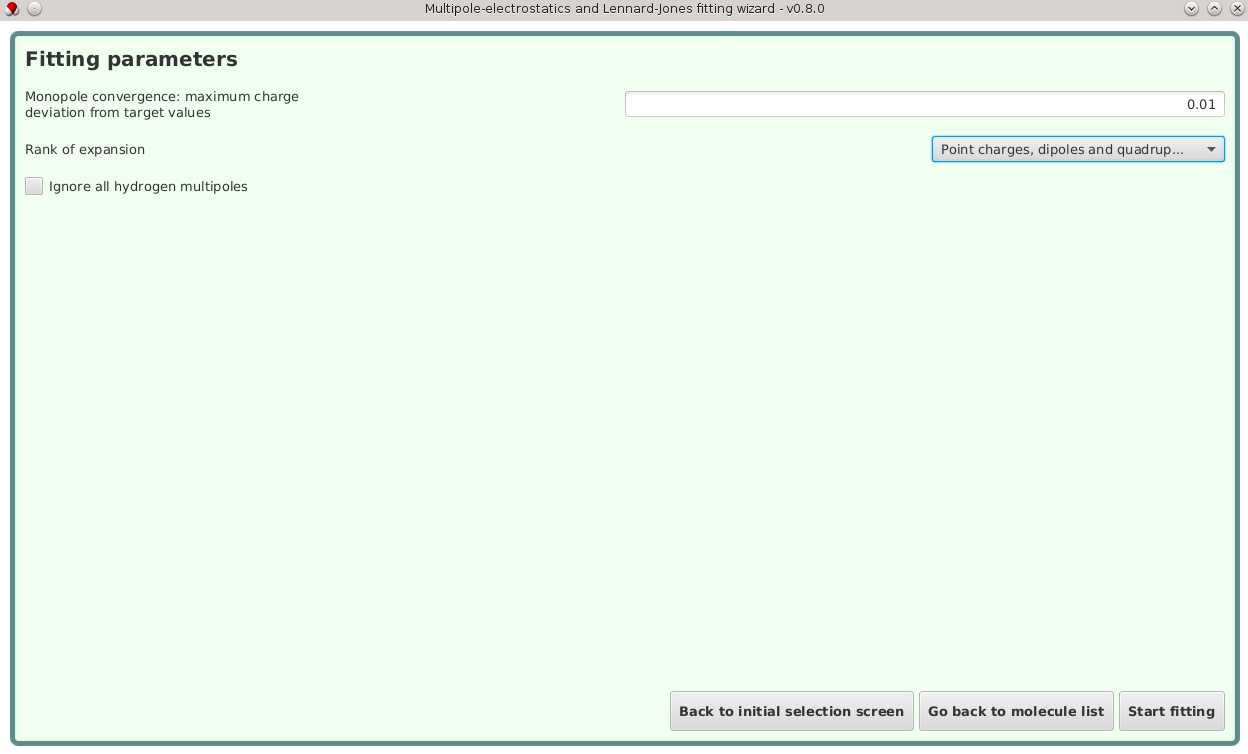
\includegraphics[width=0.9\linewidth]{pics/scr2}
\caption{Choosing fit parameters}
\label{fig2}
\end{figure}

After a short time a table displays the results : Figure \ref{fig3} \\

\begin{figure}[h!]
\centering
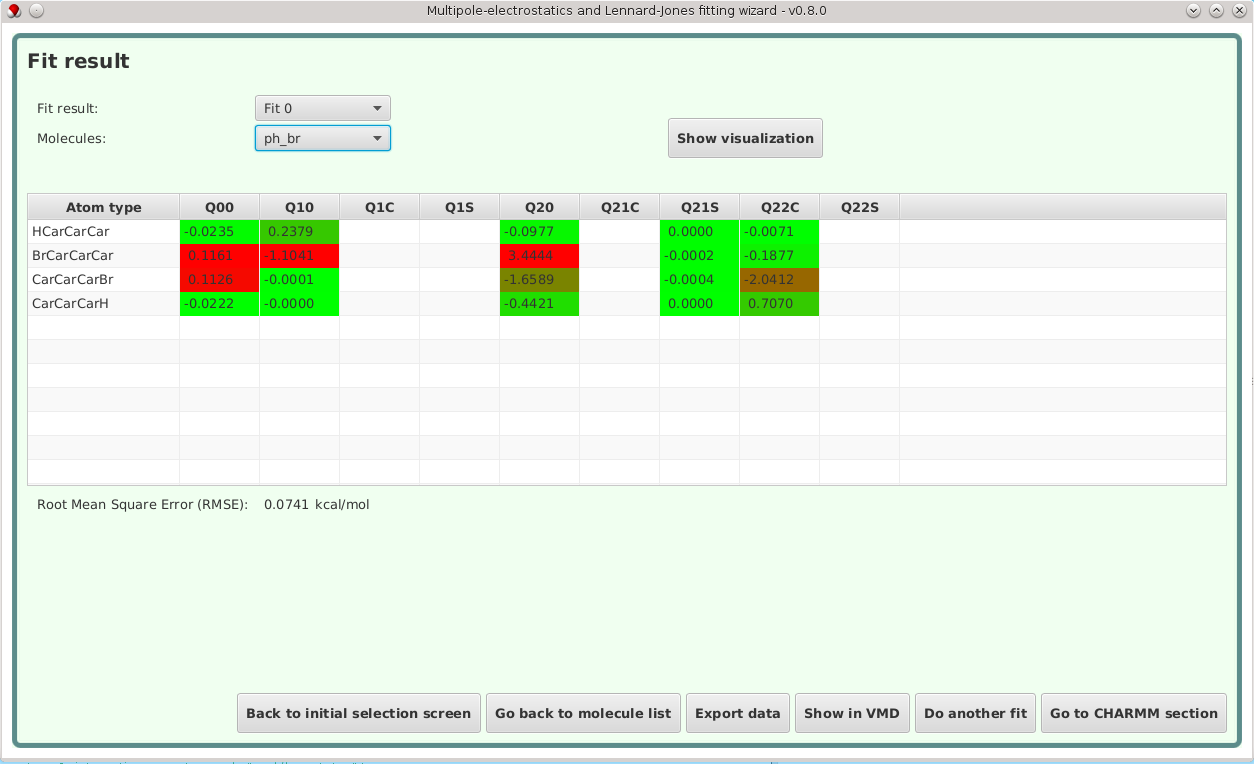
\includegraphics[width=0.9\linewidth]{pics/scr3}
\caption{Visualizing results in table}
\label{fig3}
\end{figure}

It is then possible to go to the CHARMM fit section by using the bottom right button.

\clearpage

\subsection{CHARMM fitting procedure}

From the Welcome screen (Figure \ref{fig0}) user can access directly to the CHARMM fitting 
procedure (useful if the previous section was already performed before). Otherwise the screen is 
the next step reached in the workflow : Figure \ref{fig4} \\

\begin{figure}[h!]
\centering
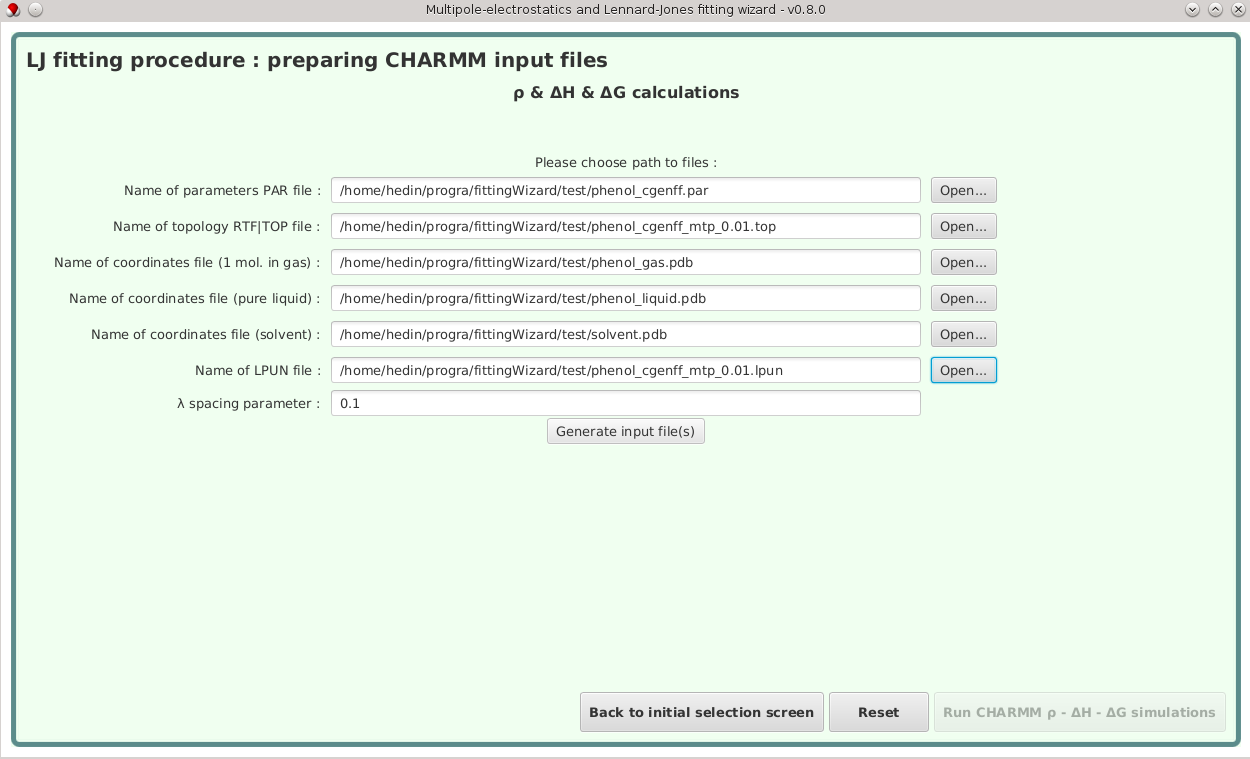
\includegraphics[width=0.9\linewidth]{pics/scr4}
\caption{CHARMM fitting procedure : choose files}
\label{fig4}
\end{figure}

\subsubsection{Generating input files}

Then input files can be generated, and they are displayed in several tabs, and if required the user 
can review and edit some of those files. When ready the user can submit all the simulations by 
pressing the bottom right button that will internally call all the required scripts : Figure 
\ref{fig5} \\

\begin{figure}[h!]
\centering
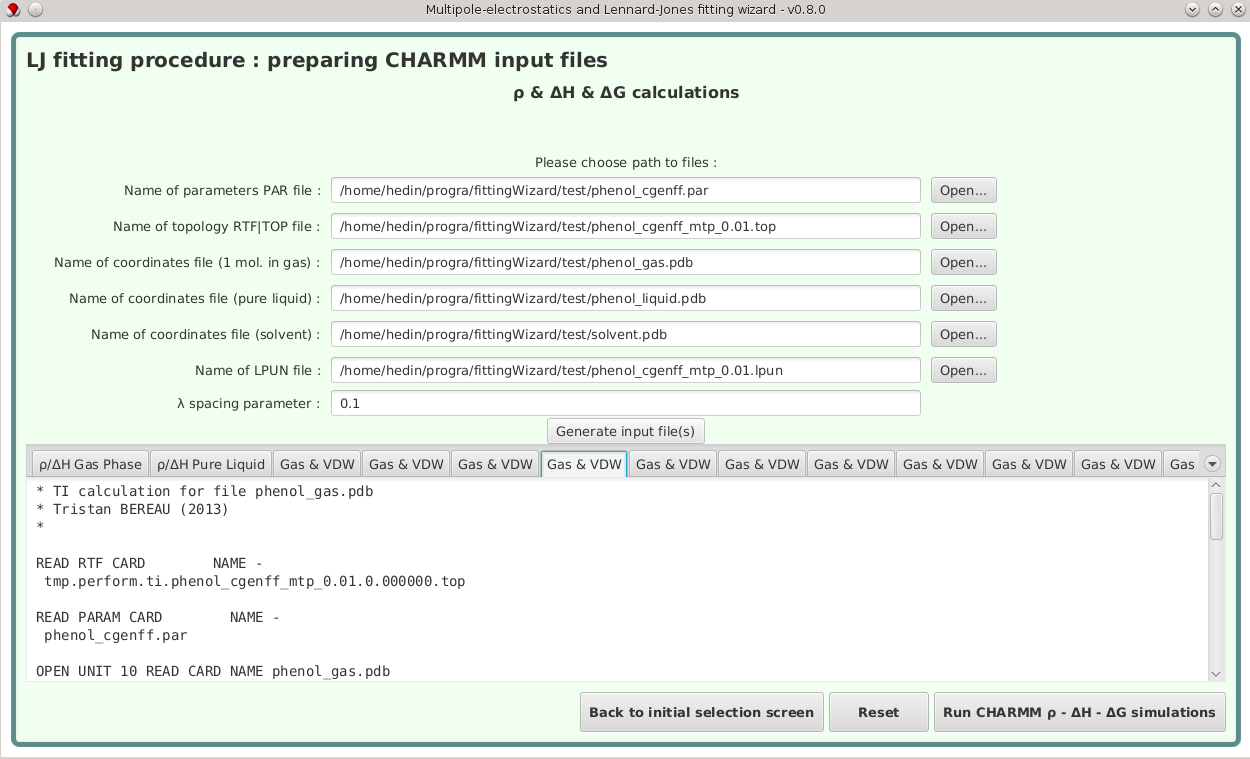
\includegraphics[width=0.9\linewidth]{pics/scr5}
\caption{CHARMM fitting procedure : all input files generated and editable if required}
\label{fig5}
\end{figure}

\subsubsection{Visualizing output files}

If for some reason simulation failed an error window appears where the user can visualize failing 
output files : Figure \ref{fig6} \\

\begin{figure}[h!]
\centering
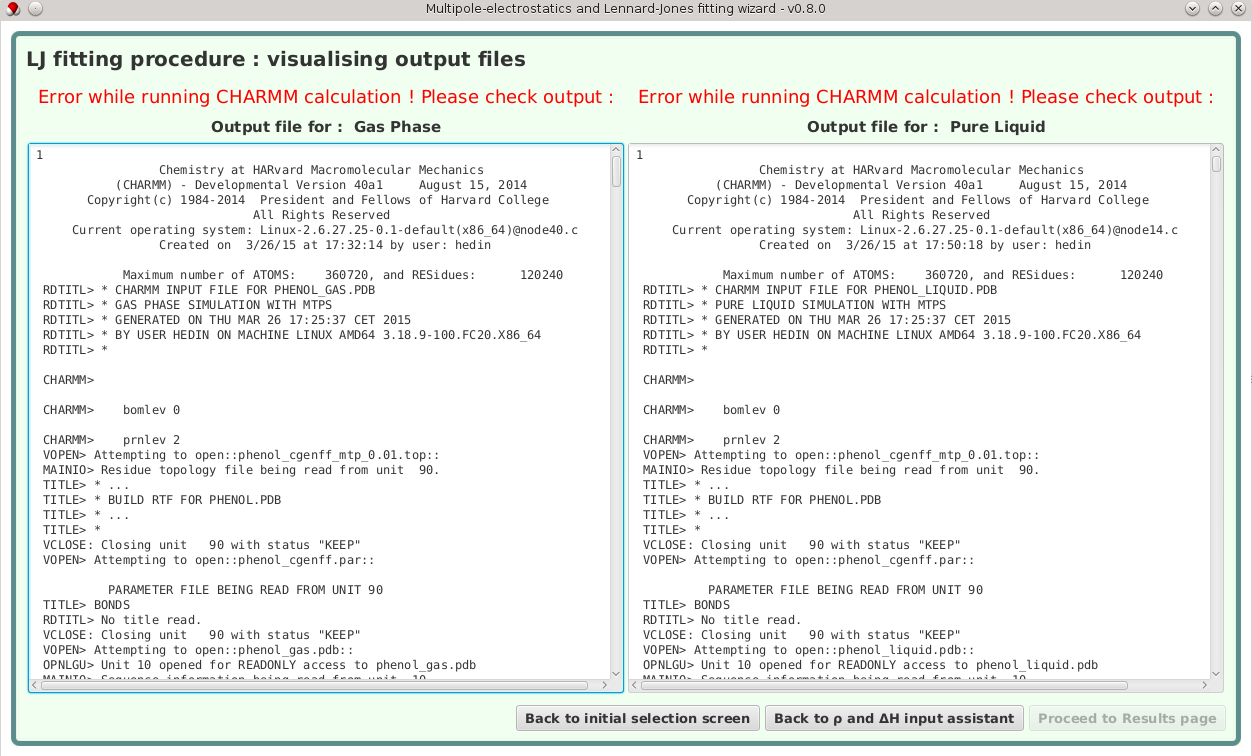
\includegraphics[width=0.9\linewidth]{pics/scr6}
\caption{CHARMM fitting procedure : error window}
\label{fig6}
\end{figure}

Otherwise at the end of all simulations the user gets a successful run window : Figure \ref{fig7}\\

\begin{figure}[h!]
\centering
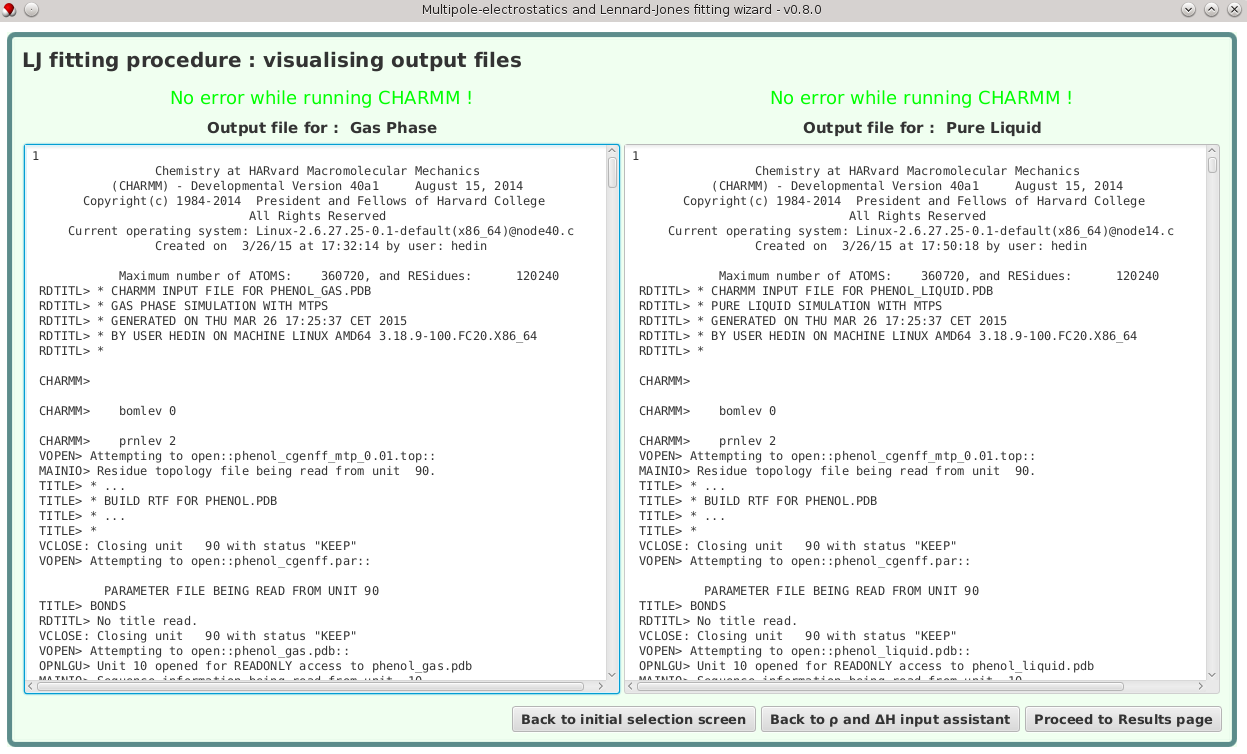
\includegraphics[width=0.9\linewidth]{pics/scr7}
\caption{CHARMM fitting procedure : success window}
\label{fig7}
\end{figure}

\subsubsection{Obtaining thermodynamic properties}

Then output files are parsed for extracting for extracting Temperature, molar mass and number of 
residues and then the density, Enthalpy of Vaporization and Free Energy of Solvation are estimated 
: Figure \ref{fig8}\\

\begin{figure}[h!]
\centering
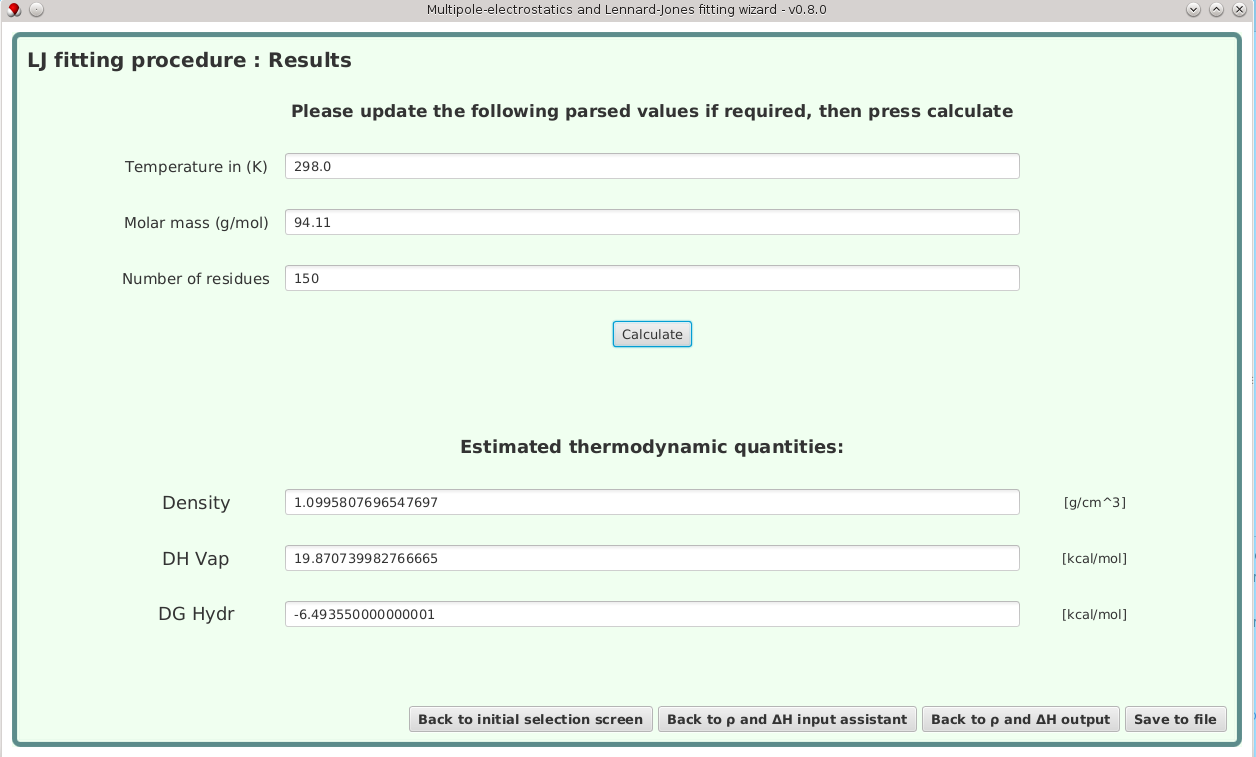
\includegraphics[width=0.9\linewidth]{pics/scr8}
\caption{CHARMM fitting procedure : obtaining the calculated thermodynamic properties}
\label{fig8}
\end{figure}

\clearpage

\subsection{Running a set of CHARMM simulations with altered PAR and TOP files}

\subsubsection{Define list of scaling parameters}

The third possibility in Welcome screen (Figure \ref{fig0}) gives the user the possibility to 
generate a set of scaled PAR and TOP files for CHARMM where the LJ parameters $\sigma$ and 
$\epsilon$ are scaled : the user first chooses how many modifications to perform : Figure 
\ref{fig9}\\

\begin{figure}[h!]
\centering
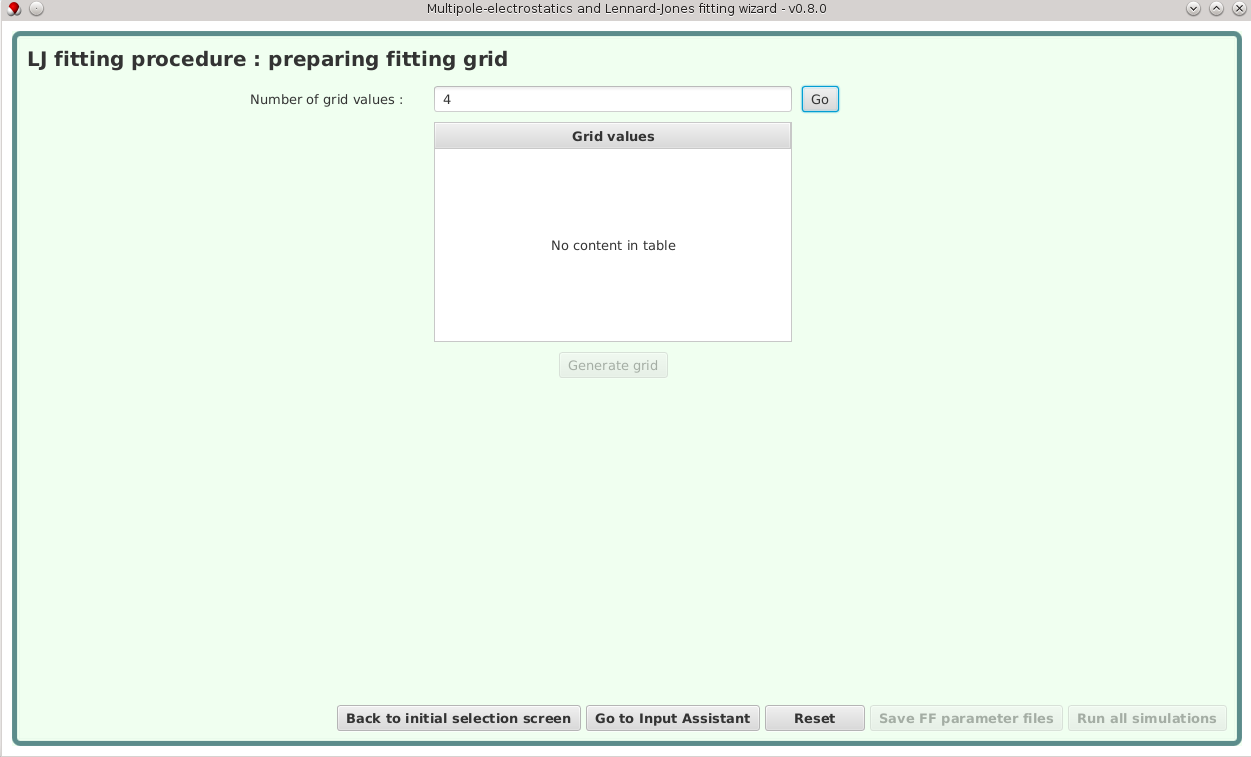
\includegraphics[width=0.9\linewidth]{pics/scr9}
\caption{CHARMM fitting procedure : defining number of grid values}
\label{fig9}
\end{figure}

Then the user chooses the scaling parameters : Figure \ref{fig10}\\

\begin{figure}[h!]
\centering
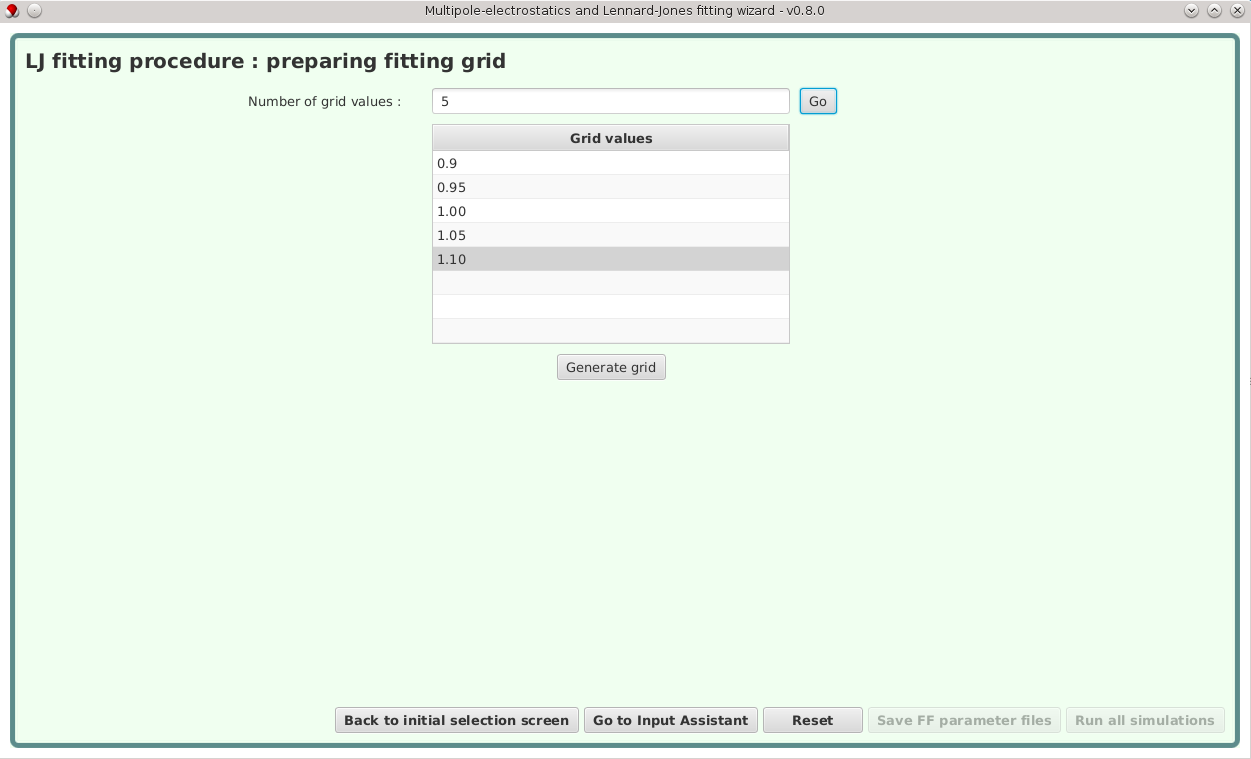
\includegraphics[width=0.9\linewidth]{pics/scr10}
\caption{CHARMM fitting procedure : defining grid values}
\label{fig10}
\end{figure}

\subsubsection{Save all files and run all simulations}

Then it is possible to save all those files an to run all simulations : Figure \ref{fig11}

\begin{figure}[h!]
\centering
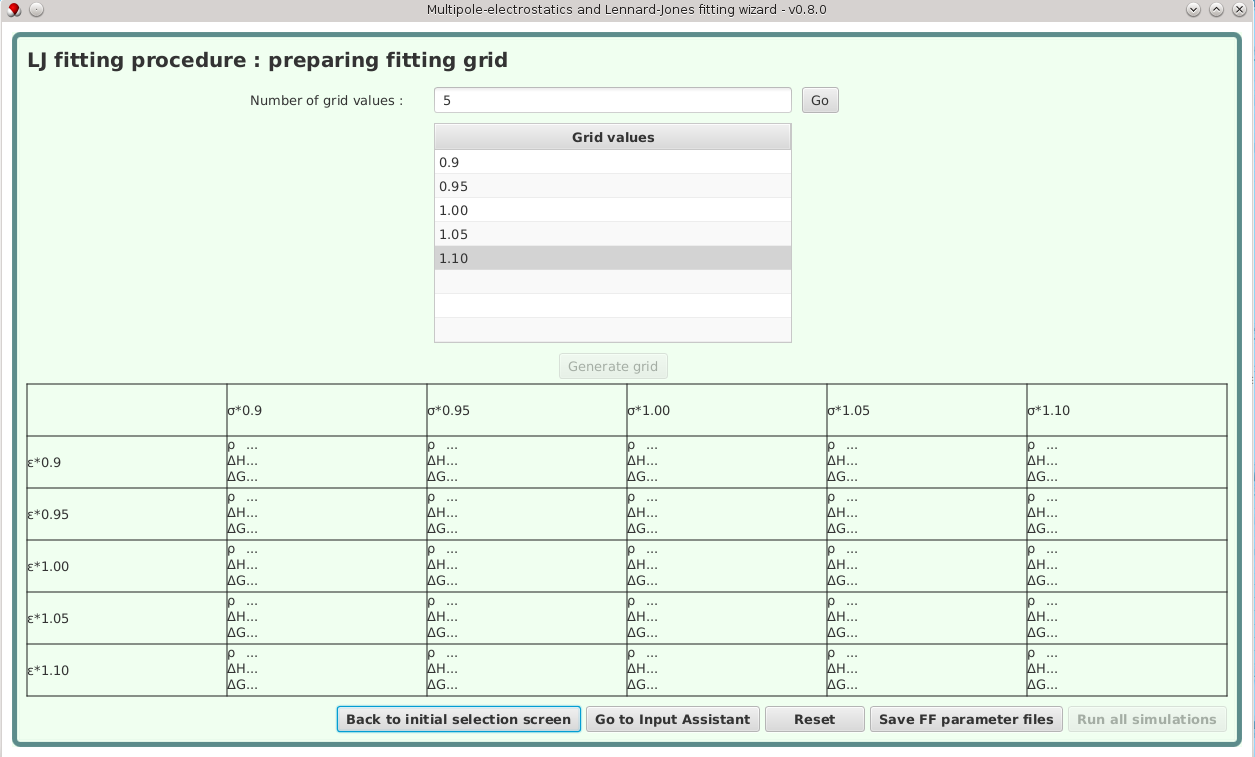
\includegraphics[width=0.9\linewidth]{pics/scr11}
\caption{CHARMM fitting procedure : saving FF files and running}
\label{fig11}
\end{figure}

\clearpage

\subsection{Generating custom PSF and TOP files using a XYZ file}

The fourth possibility in Welcome screen (Figure \ref{fig0}) gives the user the possibility to 
generate a set of custom topology (TOP,RTF) and structure (PSF) files.\\

Those files are specifically generated for the studied molecule, using the optimised XYZ 
coordinates from the Gaussian simulation.\\

Once generated the files are displayed in a tabs structure (Figures \ref{fig15} and \ref{fig16})
so the user still has the possibility to complete the generated files.

\begin{figure}[h!]
\centering
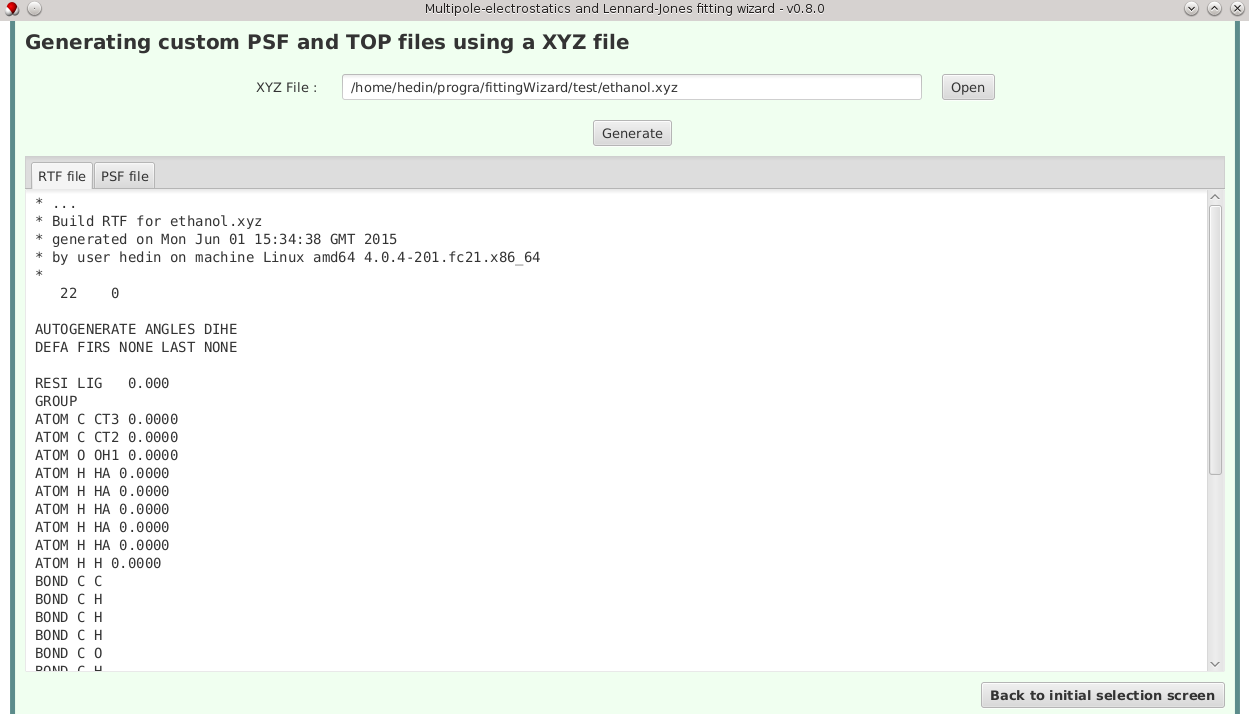
\includegraphics[width=0.9\linewidth]{pics/scr15}
\caption{CHARMM fitting procedure : generating a TOP/RTF file}
\label{fig15}
\end{figure}

\begin{figure}[h!]
\centering
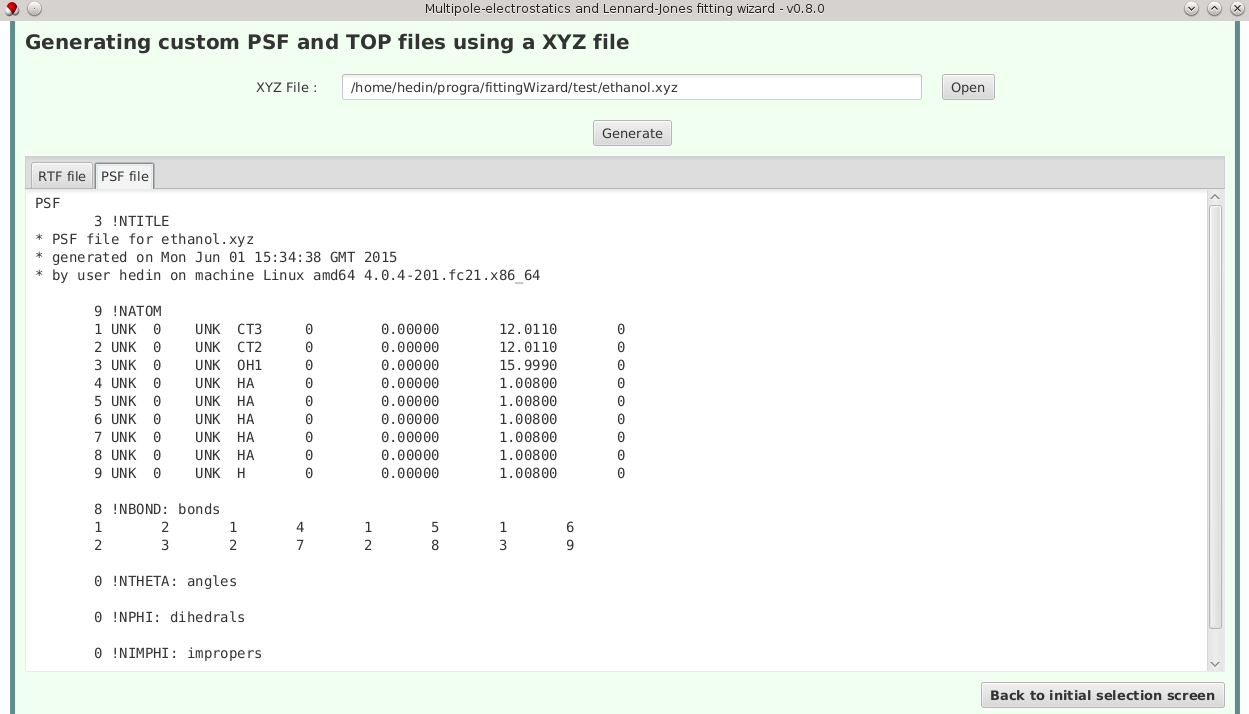
\includegraphics[width=0.9\linewidth]{pics/scr16}
\caption{CHARMM fitting procedure : generating a PSF file}
\label{fig16}
\end{figure}


\clearpage

\subsection{Database of chemical compounds}

The fifth possibility in Welcome screen (Figure \ref{fig0}) gives access to a database of 
compounds where the user can obtain experimental values for the density, Enthalpy of vaporization 
and Free Energy of solvation.\\

Compounds can be searched by : 

\begin{itemize}
\item By name : Figure \ref{fig12}
\item By formula : Figure \ref{fig13}
\item By SMILES notation : Figure \ref{fig14}
\end{itemize}

\begin{figure}[h!]
\centering
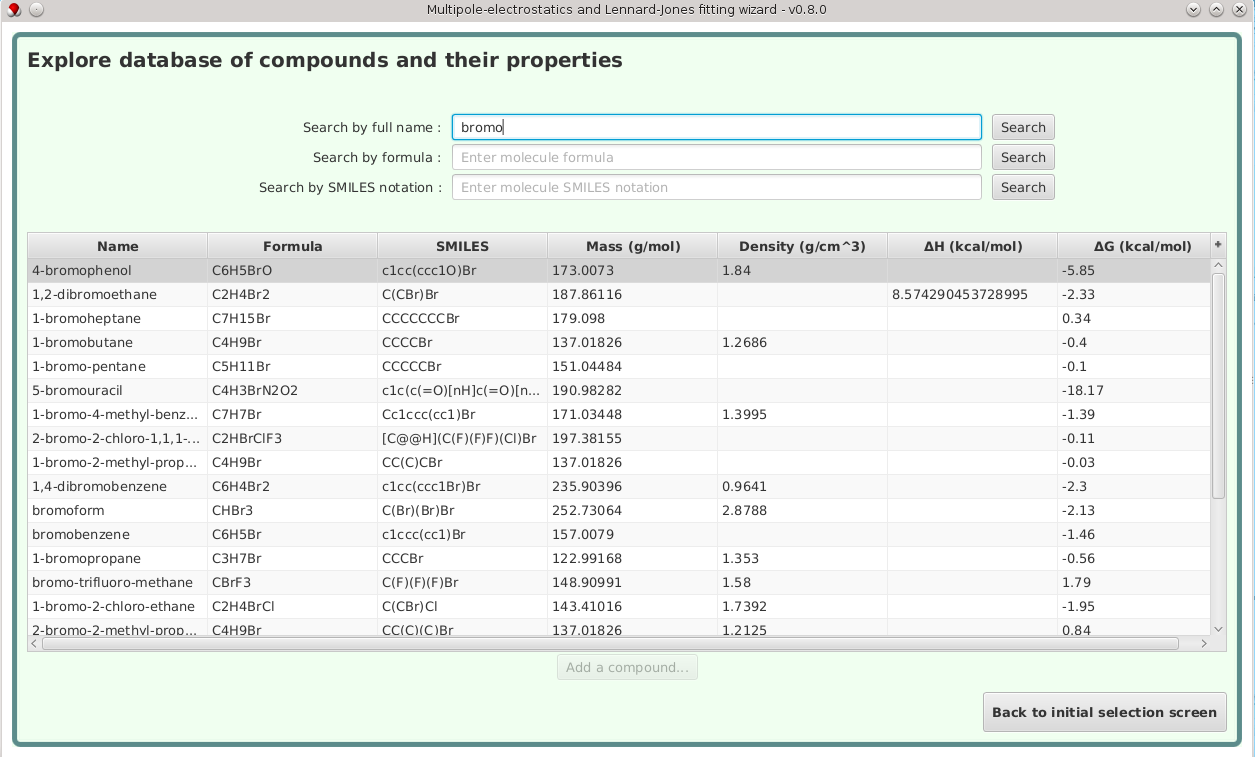
\includegraphics[width=0.9\linewidth]{pics/scr12}
\caption{Database of compounds : search by name}
\label{fig12}
\end{figure}

\begin{figure}[h!]
\centering
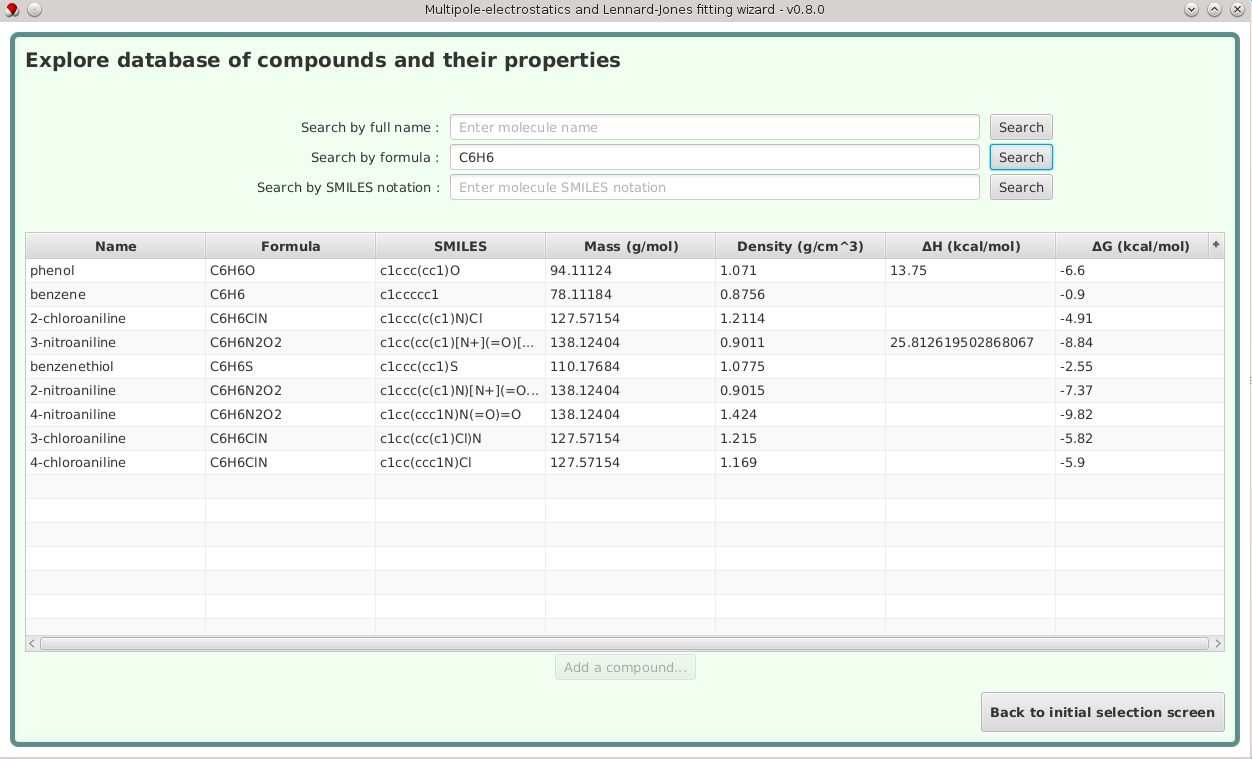
\includegraphics[width=0.9\linewidth]{pics/scr13}
\caption{Database of compounds : search by formula}
\label{fig13}
\end{figure}

\begin{figure}[h!]
\centering
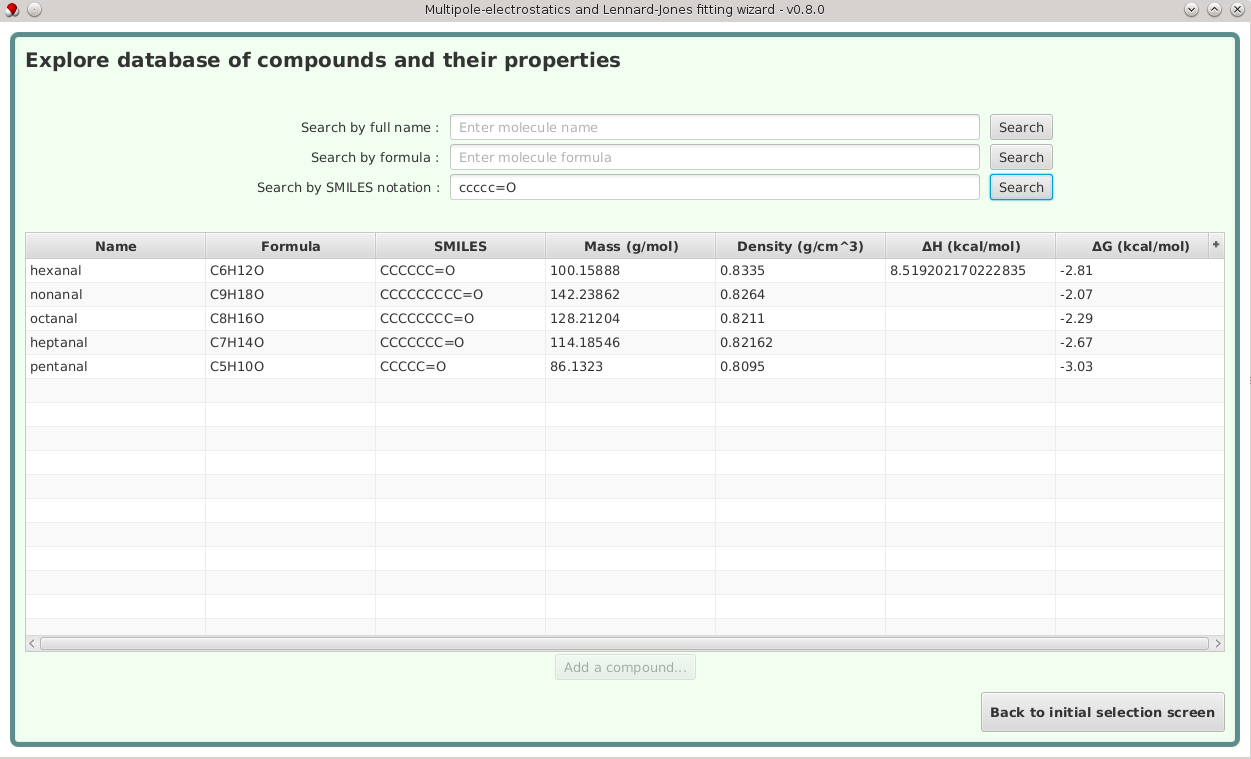
\includegraphics[width=0.9\linewidth]{pics/scr14}
\caption{Database of compounds : search by SMILES notation}
\label{fig14}
\end{figure}

\clearpage

%-------------------------------------------------
%-------------------------------------------------

%\section{Future improvements}
%
%...

%-------------------------------------------------
%-------------------------------------------------

\section{Database details}

We provide as an experimental feature the access to a database of 
mass -- density -- Enthalpy of Vaporization -- Free Energy of solvation, where the user can search 
for a molecule and get those values for then comparing to results of the CHARMM simulations.\\

The user can search molecules by name, formula or SMILES notation 
\href{http://en.wikipedia.org/wiki/Simplified_molecular-input_line-entry_system}{Wikipedia 
details}.\\

Mass, Density come from \href{https://pubchem.ncbi.nlm.nih.gov/search/}{PubChem}, Free Energy by 
results provided by David Mobley et al. (\href{http://escholarship.org/uc/item/6sd403pz}{Link})\\

The current database was designed using the \href{http://en.wikipedia.org/wiki/SQL}{SQL} 
language, see Figure \ref{dbFig} for a description of the tables an relationship between them.\\

The database is accessed either by : 
\begin{itemize}
\item As an embedded file provided with the software that is accessed using the 
\href{http://www.sqlite.org/}{SQLite} software.
\item Or as a \href{http://www.mysql.com/}{MySQL} database that is hosted on a server and then 
accessed by Local or Internet connection.
\end{itemize}

The server database is read only, and the local database should be read/write (for the moment only 
read access is provided), so that the user can easily add new molecules, add missing values, 
etc...\\

Ideas of improvements :
The user should have the possibility to ``propose'' new compounds or new values to the 
development team, then the online server-hosted database could grow interactively (of course after 
a checking procedure).

\begin{figure}[h!]
\centering
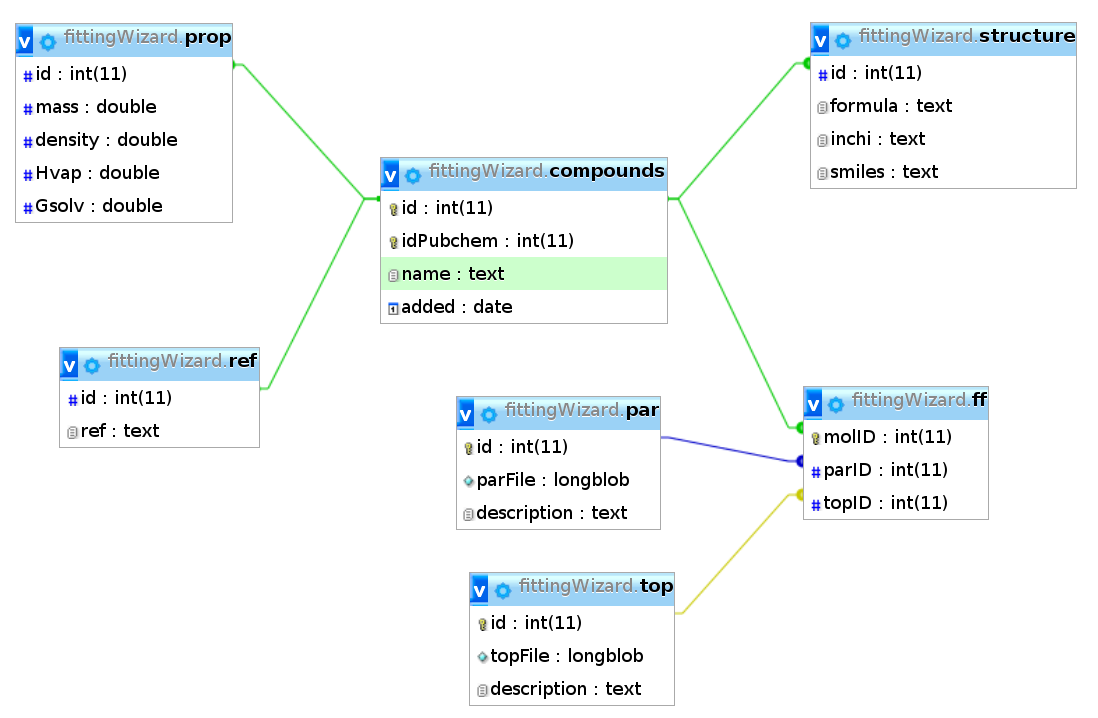
\includegraphics[width=0.9\linewidth]{pics/db}
\caption{Database of compounds : Design and relations}
\label{dbFig}
\end{figure}

%-------------------------------------------------
%-------------------------------------------------

\section{List of known Bugs}

\subsection{From the GUI}

\begin{itemize}
\item PDB : The Gaussian coordinates are saved to a XYZ file, but for the CHARMM simulation we need 
a PDB or COR file : unfortunately PDB files generated from VMD or OpenBabel are not readable by 
CHARMM directly. A code for converting the XYZ file to PDB directly from the code is currently 
being written, it will reused code from the section generating RTF and PSF files (from Figures 
\ref{fig15} and \ref{fig16}).
\end{itemize}

\subsection{From Tristan's python scripts}

Found by Florent :
\begin{itemize}
\item PRNLEV 2 in input file while using MPI is problematic and unnecessary as this is already the 
default with newer versions of CHARMM, because the I/O is messy and then difficult to parse later.
\item with CHARMM c40a2 it is necessary to increase the value of ECHECK which is bt default 20.0 
(maximum energy fluctuation between 2 steps allowed by CHARMM, it can go over 20. with some scaled 
epsilon/sigma : maybe minimisation should be longer ?)
\item ssh submission fails if the private keys are encrypted : need to use ones which are not 
password protected. but this is unsafe, need to check python reference of this ssh module for an 
alternative. 
\end{itemize}

Found by Krystel : 
\begin{itemize}
\item the use of IC in the topology file (top,rtf) may lead to incorrect results.
\end{itemize}

%-------------------------------------------------
%-------------------------------------------------

\section{Outlook}

\begin{itemize}
\item For the moment the interface is blocked (waiting screen) as long as jobs are
running : not convenient

\item Linked to previous point : add possibility to resume properly a previous
session ("data serialization" / possibility to save the whole working session)

\item Add a proper comparison (with graphs ?) of exp. vs. calculated values

\item Add the last section that will modify the epsilon parameters with a fit and run again 
simulations.
\end{itemize}

%-------------------------------------------------
%-------------------------------------------------


\section{Results}

\subsection{Phenol}

Experimental results for phenol :

\begin{itemize}
\item $\rho$ (g/cm$^-3$) : 1.073
\item $\Delta H$ (kcal/mol) : 13.75
\item $\Delta G$ (kcal/mol) : -6.60
\end{itemize}

\medskip

Simulation: $\epsilon$ and $\sigma$ were scaled by multiplying by $1.00$ or $1.05$ or $1.10$

\begin{center}
\begin{tabular}{|c|c|c|c|c|}
\hline  &  & $\sigma$*1.00 & $\sigma$*1.05 & $\sigma$*1.10 \\ 
\hline $\epsilon*1.00$ & $\rho$ (g/cm$^-3$) & 1.099 & 0.9934 & 0.9004 \\ 
\hline  & $\Delta H$ (kcal/mol) & 19.871 & 18.4993 & 17.563 \\ 
\hline  & $\Delta G$ (kcal/mol) & -6.496 & -12.78375 & -28.96785 \\ 
\hline  &  &  &  &  \\ 
\hline $\epsilon*1.05$ & $\rho$ (g/cm$^-3$) & 1.093 & 0.9973 & 0.9068 \\ 
\hline  & $\Delta H$ (kcal/mol) & 20.19 & 18.8933 & 18.0134 \\ 
\hline  & $\Delta G$ (kcal/mol) & -3.76869 & -13.69526 & -30.26755 \\ 
\hline  &  &  &  &  \\ 
\hline $\epsilon*1.10$ & $\rho$ (g/cm$^-3$)& 1.099 & 0.9951 & 0.8999 \\ 
\hline  & $\Delta H$ (kcal/mol) & 20.604 & 18.3849 & 17.67194 \\ 
\hline  & $\Delta G$ (kcal/mol) & -3.74234 & -14.03508 & -32.66905 \\
\hline  &  &  &  &  \\ 
\hline 
\end{tabular} 
\end{center}

Discussion : \\


The evolution of $\rho$ and $\Delta H$ looks coherent, but the estimates of 
$\Delta G$ are, for scaled  $\sigma$, really reaching non realistic values. One need to investigate 
scaling factors lower than one to see if such things also happen in that case.\\



Nevertheless, all the $\rho$ - $\Delta H$, and also the $\Delta G$ for $\sigma$*1.00, are similar 
to results obtained by from Prashant (unpublished work : Thermodynamic study of the intercalation 
process for various
pharmacaphore in the chromatographic system).

\end{document}
























